% !TEX root = 研究结果报告.tex
\documentclass[UTF8,zihao=-4,a4paper,fontset=fandol]{ctexart}
\usepackage[margin=24mm,headheight=15pt]{geometry}
\usepackage{amsmath,amssymb,bm,booktabs,array,tabularx,longtable}
\usepackage{graphicx,xcolor,enumitem,fancyhdr,hyperref,listings}
\hypersetup{colorlinks=true,linkcolor=blue!45!black,citecolor=blue!45!black,urlcolor=blue!45!black,breaklinks=true,hypertexnames=false}
\setcounter{tocdepth}{1}
\hypersetup{bookmarksdepth=2}
\setlength{\parindent}{2em}
\setlength{\parskip}{3pt}
\linespread{1.22}
\setlength{\emergencystretch}{2em}
\setlist{nosep,leftmargin=2em,topsep=4pt}
\renewcommand{\arraystretch}{1.18}
\setlength{\tabcolsep}{4pt}
\newcolumntype{Y}{>{\raggedright\arraybackslash}X}
\newcolumntype{P}[1]{>{\raggedright\arraybackslash}p{#1}}
\newcommand{\R}{\mathbb R}
\newcommand{\ind}{\mathbf 1}
\newcommand{\sg}{\operatorname{sg}}
\newcommand{\code}[1]{\texttt{\detokenize{#1}}}
\newcommand{\smalltable}{\small\renewcommand{\arraystretch}{1.18}}
\lstset{basicstyle=\ttfamily\small,breaklines=true,columns=fullflexible,keepspaces=true,showstringspaces=false,frame=single,rulecolor=\color{black!20},xleftmargin=0.5em,xrightmargin=0.5em}
\pagestyle{fancy}\fancyhf{}
\fancyhead[L]{\small ParallelBayes}\fancyhead[R]{\small 中文 v4 一致版}
\fancyfoot[C]{\thepage}
\ctexset{section={format=\Large\bfseries},subsection={format=\large\bfseries},subsubsection={format=\normalsize\bfseries}}
% Generated from a verified scalar bundle; do not edit numbers by hand.
\newcommand{\PBCompactValid}{3741}
\newcommand{\PBCompactNumerical}{42}
\newcommand{\PBCompactUnclassified}{105}
\newcommand{\PBCompactFunctionRows}{14981}
\newcommand{\PBCompactHighRhat}{5000}
\newcommand{\PBCompactUndefinedRhat}{1290}
\newcommand{\PBCPURWMMin}{0.424}
\newcommand{\PBCPURWMMax}{1.178}
\newcommand{\PBCPURWMAbove}{7}
\newcommand{\PBCUDARWMMin}{0.953}
\newcommand{\PBCUDARWMMax}{1.659}
\newcommand{\PBCUDARWMAbove}{14}
\newcommand{\PBCPUMALAMin}{0.116}
\newcommand{\PBCPUMALAMax}{0.394}
\newcommand{\PBCPUMALAAbove}{0}
\newcommand{\PBCUDAMALAMin}{0.234}
\newcommand{\PBCUDAMALAMax}{0.408}
\newcommand{\PBCUDAMALAAbove}{0}


\hypersetup{pdftitle={ParallelBayes 研究结果报告：中文v4一致版},pdfauthor={ParallelBayes项目}}
\begin{document}
\begin{titlepage}\centering
\vspace*{18mm}
{\LARGE\bfseries ParallelBayes\par}
\vspace{10mm}
{\huge\bfseries 研究结果报告\par}
\vspace{5mm}
{\Large 时间执行成本、后验探索与可重建证据\par}
\vspace{12mm}
{\large 中文 v4 一致版\par}
{\large 2026年10月12日\par}
\vspace{16mm}
\begin{minipage}{.87\linewidth}
\textbf{报告范围。}完整说明研究软件的能力、主实验设计、数值核验、成本与误差结果，以及 H1/L2/W1 和 CPU NUTS 的有限补充。历史与正式批次分别解释。

\textbf{证据绑定。}科学结论与封存中文 v4 正文、补充材料和完整结果附录一致。所有结果来自既有计算及已验收分析；本次整理未增加正式采样、GPU测试或新参考点。

\textbf{阅读提示。}“数值有效”表示满足指定输出标准，“推断可靠”还取决于探索、函数和参考。“更快”须注明同核、设备和成本边界；本报告保留未达标与未分类失败。
\end{minipage}
\vfill
{\small 配套材料：研究计划、中文 v4 正文、SI及完整结果附录。\par}
\end{titlepage}
\pagenumbering{roman}
\tableofcontents\clearpage
\section*{术语与缩写}
\addcontentsline{toc}{section}{术语与缩写}
\noindent\begin{tabularx}{\linewidth}{P{34mm}Y}\toprule
缩写/术语 & 本文含义\\\midrule
MCMC & 马尔可夫链蒙特卡洛\\
RWM & 随机游走 Metropolis 核\\
MALA & Metropolis 校正 Langevin 核\\
NUTS & 无折返采样器；此处为成熟外部基线\\
MSE / RMSE & 均方误差 / 均方根误差\\
MCSE & 蒙特卡洛标准误，描述有限计算的不确定性\\
ESS & 有效样本量；不等于独立实验重复数\\
ESJD & 期望平方跳跃距离；开发选择使用其样本估计\\
JVP & 雅可比—向量积；quasi-DEER 的代理导数计算\\
SBC & 基于模拟的校准，重复先验生成与数据拟合\\
BCa & 偏差校正与加速的 bootstrap 区间\\
IID & 独立同分布；稀有事件例中只作明确假想参照\\
数值有效 & 通过指定数组、路径及输出契约检查，不自动等于后验探索充分\\
参考平方差 & 相对有限数值/采样参考的平方差，不自动等于真值 MSE\\\bottomrule
\end{tabularx}
\clearpage

\pagenumbering{arabic}

\section{研究结论与证据范围}
\subsection{主要发现}
ParallelBayes 提供可核对实际随机输入的研究软件，将目标、转移核、执行器及计量策略分开。在指定 Windows CPU/CUDA 条件下，Online Picard 的普通工作流配对几何平均速度比为 CPU \PBCPURWMMin--\PBCPURWMMax、CUDA \PBCUDARWMMin--\PBCUDARWMMax；quasi-DEER 为 CPU \PBCPUMALAMin--\PBCPUMALAMax、CUDA \PBCUDAMALAMin--\PBCUDAMALAMax。quasi-DEER 所有组均慢于配对顺序实现，Picard 的部分点估计更快。速度比以顺序耗时除以并行耗时定义，不代表后验推断加速。

正式3888项主任务中，\PBCompactValid 项满足规定数值标准，\PBCompactNumerical 项数值失败，\PBCompactUnclassified 项未分类失败，均保留。独立重放的有效 MH 与缓存转移共有54,448,128次，接受事件失配为零。数值一致与充分探索并不等价：有效拟合的14,981个所选函数诊断行中，5000行有有限 $\hat R>1.01$，1290行未定。诊断行不是独立实验数量。

水井 W1 在4096步预算下提供有用的连续函数比较；MALA较RWM有更小参考平方差，但时间执行器增加其普通成本。多峰 M1 的均衡初始化能使池化符号比例接近真值，即使几乎没有保存的跨峰移动。L2/W1 的极稀有符号事件全零，在绝对平方差上可以很小，却相对正概率参考有100\%误差；全零本身不能诊断混合不良。

\subsection{成立的贡献及其限度}
本研究的增量是可重用的软件与实际输入核验流程，以及指定实现下对成本、探索和参考精度的计算证据。既有研究已提供 quasi-DEER/Picard 机制及时间并行软件\cite{zoltowski,grazzi,gonzalez,parallelmcmc}，已有跨引擎工具和 R 加速接口\cite{comparemcmcs,bayesforge}。统一 R 接口、框架 CUDA 探测或任务数量本身不承担创新论证。

正式紧凑主研究的比较针对固定维度连续目标、当前窗口适配、1024/4096两个预算及指定资源条件；历史批次、较长参考计算与有限补充保持各自身份。没有得出普遍 CPU/CUDA 加速、所有目标收敛、精确达标时间或全部历史失败已解决的结论。当前研究计算与内部复现验收完成，材料的外部访问及期刊投稿仍需作者决策。

\section{软件与执行器的数学对象}
\begin{table}[htbp]\centering\smalltable
\begin{tabularx}{\linewidth}{P{36mm}Y Y Y}\toprule
目标入口及设备 & 顺序 RWM/MALA & Picard RWM、quasi-DEER MALA & NUTS\\\midrule
Stan/BridgeStan，Mac CPU & 支持 & 不支持 & 不支持\\
明确原生 JAX 目标，CPU & 支持 & 支持对应组合 & BlackJAX 基线\\
明确原生 torch 目标，Windows CPU & 已核验 & 已核验，含主机控制 & 独立 Pyro 研究 CLI\\
明确原生 torch 目标，Windows CUDA & 已核验 & 已核验，含主机控制 & 未接入或核验\\\bottomrule
\end{tabularx}
\caption{v4 对应的软件能力与实际设备边界。原生 Windows Stan 编译尚未核验。Pyro 四进程基线不属于通用 \code{pb_sample()} 的 torch NUTS 选项，也不是 NUTS 轨迹的时间并行。}
\end{table}

\code{pb_capabilities()} 查询包接口组合；独立研究 CLI 的契约另列。\code{pb_benchmark()} 运行配置列表并组织 R 结果，完整冻结协议、任务恢复和原始证据管理由 Python CLI 及项目文件完成。Stan 入口没有默认独立轨迹参考，\code{audit=TRUE} 明确拒绝。扩展目标需提供原生 Python 模型及独立参考，不支持把任意 Stan 文件自动编译为 JAX/torch GPU 目标，也不是任意 R 闭包的一键时间并行接口。

\subsection{目标、坐标与实际随机输入}
设原参数为 $\theta=T(q)$，$T$ 是相应自由坐标之间的可微一一变换，实际计算使用 $q\in\R^d$。计算目标为
\begin{equation}\label{eq:target}
\ell(q)=\log p(y,T(q))+\log|\det J_T(q)|.
\end{equation}
约束变换、参数顺序和 Jacobian 项共同决定目标分布。两个实现若省略不同的参数无关常数，核对 $\ell(q)-\ell(q_0)$，而非要求原始对数密度相等；梯度必须在同一坐标下比较。正值测试使用 $\theta=e^q$ 及 lognormal 密度，并通过故意遗漏 Jacobian 检查测试系统的敏感性。

固定初值、核参数、提议噪声和均匀随机数组后，MCMC 成为确定递推 $q_t^\star=F_t(q_{t-1}^\star)$。配对执行器读取同一实际数组；两个软件设置同一整数种子并不能替代这项控制。采样数组由锁定 NumPy 版本的 Philox 生成，导数探针另用随机流，数组及哈希一并保存。独立 NumPy 顺序参考使用独立密度、解析梯度和显式循环，不调用待核验的 JAX 或 torch 转移函数。

\subsection{两种转移核}
随机游走 Metropolis（RWM）使用 $q'=q+s z$，$z\sim N(0,I_d)$，对数接受比为 $a=\ell(q')-\ell(q)$。Metropolis 校正 Langevin 算法（MALA）使用
\begin{align}
q'&=q+h\nabla\ell(q)+\sqrt{2h}\,z,\\
a(q,q')&=\ell(q')-\ell(q)-
\frac{\|q-q'-h\nabla\ell(q')\|^2-\|q'-q-h\nabla\ell(q)\|^2}{4h}.
\end{align}
当 $\log u<a$ 时接受，否则保留 $q$；拒绝自环仍计为一次转移。这里 $h$ 不是提议噪声的标准差。NUTS 基线保留自身随机流与适应预热，不与 MH 核共享整条路径。

\subsection{窗口 quasi-DEER MALA}
在固定输入下，窗口内第 $k+1$ 轮路径满足
\begin{equation}\label{eq:deer}
q_t^{(k+1)}=F_t(q_{t-1}^{(k)})+
B_t^{(k)}\{q_{t-1}^{(k+1)}-q_{t-1}^{(k)}\}.
\end{equation}
旧路径上的映射和 $B_t^{(k)}$ 可批量计算，再将右侧整理为仿射递推，通过结合扫描求解。精确算术下，若各映射有定义、$B$ 有限且扫描被精确求解，第 $k$ 轮至少恢复前 $k$ 个状态，长度 $W$ 的窗口至多经过 $W$ 轮恢复原递推\cite{gonzalez,zoltowski}。固定窗口起点使第一步正确；前 $k$ 步正确时，下一轮保持这段前缀，第 $k+1$ 步的修正项为零。这一因果性质不要求 $B$ 是真实 Jacobian，也不保证浮点实现提前停止后的路径精度。

实际实现将硬接受变量 $b=\ind\{\log u<a\}$ 与软门控组合：
\begin{equation}
g=b+\sigma(a-\log u)-\sg\{\sigma(a-\log u)\},\qquad
B_t=\operatorname{Diag}\!\left[\operatorname{clip}\{v_t\odot(J_{\rm proxy,t}v_t),-1,1\}\right].
\end{equation}
前向仍使用硬 MH 输出；torch 另以停止梯度构造避免软项的舍入抵消。$J_{\rm proxy}$ 是代理 Jacobian，而非硬 MH 映射的真实导数。每链每位置一个 Rademacher 探针 $v_t$，在窗口迭代中复用；截断仅作用于导数近似。

原论文伪代码的软门控使用 $\sigma(\min(0,a)-\log u)$；本项目归档上游提交 \code{5e5b637} 及适配实现使用未截断的 $a$。硬接受判据等价，代理导数一般不同。此外，本研究使用非重叠窗口、重复窗口起点的初猜和硬残差停止，不使用 NaN 归零或状态裁剪。因此性能结论属于所测适配实现，不能视为原实现的直接复现。

\subsection{Online Picard RWM}
对于已经确认的窗口起点 $q_L$，先计算固定噪声对应的接受增量，再通过前缀和重建候选路径\cite{grazzi}：
\begin{align}
D_t^{(k)}&=s z_t\ind\{\log u_t<\ell(q_{t-1}^{(k)}+s z_t)-\ell(q_{t-1}^{(k)})\},\\
q_t^{(k+1)}&=q_L+\sum_{i=L+1}^{t}D_i^{(k)}.
\end{align}
在新路径的前驱处重新计算接受事件，只提交连续一致的最长前缀。若四个位置依次为“一致、一致、不一致、一致”，只能提交前两个位置，第四个位置的前驱尚未确认。torch 多链按各链确认长度的最小值共同推进，末尾窗口使用实际剩余长度。浮点前缀和与顺序加法可能不同，事件匹配仍需配合独立路径核对。

\subsection{数值输出标准}
quasi-DEER 的窗口停止检查硬递推残差；Picard 使用前述连续前缀确认。残差条件为
\begin{equation}
\max_{t,j}\frac{|q_{t,j}-F_t(q_{t-1})_j|}
{\mathrm{atol}+\mathrm{rtol}|F_t(q_{t-1})_j|}\leq1.
\end{equation}
正式审计另按每链检查最大路径差不超过
$100[\mathrm{atol}+\mathrm{rtol}\max(1,\max_{t,j}|q_{t,j}|)]$，其中两项容差均为 $10^{-10}$；接受事件失配必须为零。局部残差小不推出长路径误差小，代理导数也不是后验偏差证明。历史判据使用链内整体状态尺度，后续逐函数分析补充其含义，未追溯修改资格。

非有限值、迭代耗尽和外部路径失配都保留为失败，失败数组不能转为正式后验样本。本版将非有限提议密度统一视为失败，尚未一般区分合法支持集外 $-\infty$ 与 NaN/计算异常；这一处理限制支持范围。主研究未用重抽随机数、删除困难状态或顺序回退改变资格。


\section{正式研究设计与统计口径}
\subsection{正式模型库与坐标}
正式研究包括九个目标、36 个预先指定的后验函数。为便于数值核对与解释，区分基础模型坐标 $r$、实际采样坐标 $q$ 和输出参数 $\theta$：$r=c+Lq$，$\theta=T_0(r)$；目标含 $\log|\det L|$ 及所需约束项。

\begin{table}[htbp]\centering\smalltable
\begin{tabularx}{\linewidth}{l r Y Y}\toprule
目标 & 维数 & 模型与数据 & 坐标及比较作用\\\midrule
G1 & 8 & 标准正态 & $c=0,L=I$；解析控制\\
G2 & 64 & 旋转高斯，原协方差条件数100 & 完整 Cholesky 白化；高维稠密计算\\
A1 & 64 & 潜在 AR(1)，$\rho=0.9$，单位观测噪声 & 后验均值平移与完整白化\\
L1 & 8 & logistic，$n=256$，先验标准差2.5 & 众数及观测信息坐标\\
L2 & 8 & logistic，$n=4096$，同一生成系数 & 似然成本及极稀有事件\\
H1 & 9 & 中心化漏斗，$v\sim N(0,9)$ & 原坐标，检验几何与路径敏感性\\
H2 & 9 & 非中心化漏斗 & 输出回原尺度，核随坐标改变\\
M1 & 8 & $\frac12N(-5e_1,I)+\frac12N(5e_1,I)$ & 双峰探索与分散初始化\\
W1 & 2 & 水井真实数据，3020条 & 截距、距离系数；二维参考\\\bottomrule
\end{tabularx}
\caption{当前 v4 的正式目标库。完整数据、矩阵、浮点配置及哈希随冻结协议保存。}
\end{table}

G2 的协方差为 $\Sigma=U\Lambda U^\mathsf T$，$\Lambda_{jj}=100^{(j-1)/63}$，$U$ 来自固定正态矩阵的 QR 分解。A1 的先验协方差为 $K_{ij}=0.9^{|i-j|}$，固定数据后 $\Sigma=(K^{-1}+I)^{-1}$、$m=\Sigma y$。二者在实际 $q$ 坐标均为标准正态，原尺度相关性不能直接解释本轮核的混合差异。

L1/L2 的设计含截距及七列标准化正态变量，系数先验为 $N(0,2.5^2)$，生成系数相同但数据不同。W1 为
$\Pr(y_i=1)=\sigma(\alpha+\beta d_i/100)$，在两个系数上用平坦先验。三种回归目标从零点开始，以 trust-exact 求众数；目标有限且解析梯度最大绝对值不超过 $10^{-7}$ 时接受，最多300步，$L$ 为观测信息逆矩阵的 Cholesky 因子。未做特征值修复，也未用参考样本构造坐标；该变换不把 Laplace 近似当作后验真值。

H1 为 $x_i\mid v\sim N(0,e^v)$，$i=1,\ldots,8$；H2 使用独立 $z_i\sim N(0,1)$ 并输出 $x_i=z_i e^{v/2}$。两者表示同一原尺度后验，但在各自坐标使用同一数值步长并不意味着同一原尺度转移核。

\subsection{独立开发选择与冻结配置}
步长在正式输入之外选择。RWM 候选为 $\{0.5,1,1.5,2.4,3.5,5\}/\sqrt d$；MALA 候选为 $\{0.1,0.3,0.6,1,1.6,2.4\}/d^{1/3}$。每候选两份四链输入，丢弃512步、保留1024步；仅在两次均有效时，以平均 ESJD/$d$ 最大者入选，平局取较小步长。该准则衡量局部移动，未优化 ESS 或稀有事件精度。

\begin{table}[htbp]\centering\smalltable
\begin{tabular}{lrrl}\toprule
目标 & MALA $h$ & RWM $s$ & 固定中心及线性变换\\\midrule
G1 & 0.8 & 0.848528137 & $0,I$\\
G2 & 0.4 & 0.3 & $0,\operatorname{chol}(\Sigma)$\\
A1 & 0.4 & 0.3 & $m,\operatorname{chol}(\Sigma)$\\
L1/L2 & 0.8 & 0.848528137 & 众数及观测信息\\
H1 & 0.480749857 & 1.66666667 & $0,I$\\
H2 & 0.769199771 & 0.8 & $0,I$\\
M1 & 0.8 & 0.848528137 & $0,I$\\
W1 & 1.26992084 & 1.69705627 & 众数及观测信息\\\bottomrule
\end{tabular}
\caption{冻结配置的显示精度。归档 JSON 提供完整精度；$h$ 对应噪声 $\sqrt{2h}$，$s$ 是 RWM 提议标准差。}
\end{table}

开发批次216项中212项完成，4项 H1 MALA 失败保留。H1 RWM 选择了候选上边界，说明配置仍受有限搜索范围约束。已记录开发任务内部成本226.917秒、坐标构造0.128秒；其中包含审计及写盘，未包含新进程导入，不能直接并入或扣除正式普通调用成本。

\subsection{正式网格、预算与资源}
每目标24份独立四链实际输入；同核的两个执行器及两设备读取同一输入。九种工作流为 CPU/CUDA 的四种 MH 组合，以及独立 CPU Pyro NUTS。两档预算每链保留1024或4096次转移，总计
\begin{equation}9\times9\times2\times24=3888\ \text{项主任务}.
\end{equation}
四链、时间执行器和设备重复不增加独立重复数。缓存探测限于 G1/G2/L2/W1，共256项、1024次调用；不计入正式后验拟合。

四链初值来自 $N(0,4I)$，M1 首坐标设为 $(-5,5,-5,5)$。MH 与 NUTS 共用初值，但 NUTS 使用独立随机流及预热。MH 丢弃512步、窗口32；quasi-DEER 每窗口最多2048轮，Picard最多 $N+512$ 轮。NUTS 用四个原生 spawn 子进程，每链预热1024步、目标接受率0.8、最大树深8，适应步长及对角质量矩阵，未使用 JIT。

正式 Windows 环境为原生 Windows 11、AMD Ryzen 7 9800X3D、RTX 5080，float64；Python 3.12.14、NumPy 2.2.6、SciPy 1.15.3、torch 2.13.0+cu130、Pyro 1.9.2、psutil 7.1.0，R 4.6.1、posterior 1.7.0。MH 进程 torch 线程4、interop线程1；NUTS每个子进程各为1。BLAS线程环境变量未统一设置，不能把这些数字解释为所有库的硬上限或独占物理核心预算。

存储/工作区估计上限2048 MiB、进程树 RSS 监督上限8 GiB、Windows Job提交内存上限12 GiB，三者计量不同。启动要求可用主存至少12 GiB、磁盘4 GiB，CUDA另需空闲显存3 GiB，运行磁盘底线1 GiB。资源不足暂停启动，数值失败、进程失败与未启动分别记录。没有总实验时限，也未通过重试或回退改变样本资格。

\subsection{函数、尺度与参考}
\begin{table}[htbp]\centering\smalltable
\begin{tabularx}{\linewidth}{l Y Y}\toprule
目标 & 原尺度上的函数集合 & 参考及其性质\\\midrule
G1/G2/A1 & 标准化首参数 $z$、$z^2$、$\ind(z>1)$ & 解析：$0,1,1-\Phi(1)$\\
L1/L2 & $\theta_1,\theta_2,\sigma(\theta_1),\ind(\theta_1>0)$ & 独立有限 NUTS；L2事件另作重要性参考\\
H1/H2 & $v/3,\tanh(v/3),\ind(x_1>0),\cos(x_1e^{-v/2})$ & 解析：$0,0,1/2,e^{-1/2}$\\
M1 & $\theta_1/\sqrt{26},\ind(\theta_1>0),\theta_2,\theta_2^2$ & 解析：$0,1/2,0,1$\\
W1 & $\alpha,\beta,\alpha^2,\beta^2,p(0),p(100),\ind(\beta>0)$ & 冻结求积点；v4另给确定数值包络\\\bottomrule
\end{tabularx}
\caption{全部36函数。各尺度 $s_f=1$，因此阈值表示函数原单位上的绝对误差，而非自动统一的相对精度。}
\end{table}

对方法 $a$ 和预算 $N$，在数值有效且函数有限的重复集合 $V$ 上计算
\begin{equation}\label{eq:loss}
\widehat E_{a,f}(N)=\frac{1}{|V|}\sum_{r\in V}
\frac{(\widehat\mu_{a,f}^{(r)}(N)-\mu_f^{\rm ref})^2}{s_f^2}.
\end{equation}
解析参考时可解释为有效输出条件下的 MSE 估计；有限参考时称为参考平方差。比较两方法固定共同有效集合，同时报告全部24份的失败分母，不以 $\hat R$ 达标筛掉困难拟合。预算点上的最大函数平方差 $\leq0.01$ 对应 RMSE $\leq0.1$，只对指定函数与尺度有意义。误差估计的 MCSE 判据与这一误差阈值分开，不把短链 ESS 当作真实 MSE。

主分析使用9999次逐点 BCa bootstrap，单位为整份四链独立输入，至少20份共同有效重复才计算区间；退化情况保留未定，不作全体比较的同时置信声明。秩正态化与折叠 $\hat R$、bulk/tail ESS 由 posterior 计算\cite{vehtari,posterior}；常量函数不填成 $\hat R=1$。预算仅两个点，报告已测预算的误差与耗时，不插值为精确达标时间。

L1/L2 每模型四份独立四链 NUTS 参考，每链预热1024、保留16384步，共262144个相关状态；MCSE取批均值与拟合间估计的较大者。无记录发散不能排除共同偏差。L2原符号事件全零，其不确定性保持未定。W1 原参考以12个保存的浮点求积配置检查稳定性；这些变化不是认证误差界。v4的 L2 重要性参考和 W1 确定包络单独报告，不覆盖原参考身份。

\subsection{成本边界与比较单位}
\begin{table}[htbp]\centering\smalltable
\begin{tabularx}{\linewidth}{l Y Y}\toprule
口径 & 包含内容 & 回答的问题\\\midrule
缓存执行 & 已准备内核的执行，显式设备同步 & 同一指定计算能否更快完成？\\
普通批量工作流 & 进程启动、输入/目标准备、预热/丢弃、采样、变换、正常结果和 R 诊断 & 获得可分析输出的实际批量成本\\
研究审计 & 再含独立路径参考、保护、完整证据归档 & 取得可核验研究材料的成本\\
R 前端技术成本 & 最外层 R 启动/依赖、结果传回与转换的实测 & R 使用者首次与重复调用的边界\\\bottomrule
\end{tabularx}
\caption{成本口径相互嵌套或属于另测边界，不能直接相加。开发调参、整库环境安装和全局归档上传另列。}
\end{table}

同设备、同核、同输入配对的速度比为 $S=T_{\rm seq}/T_{\rm par}$，$S>1$ 表示时间执行更快。不同核需结合函数误差与诊断解释。跨 Mac/JAX 和 Windows/torch 的差异同时包含硬件、后端及实现，不归因于算法单一因素。批处理向量化不等于已证明物理核心有效利用；CPU/CUDA计时包含实际同步及主机控制成本。


\section{数值核验、失败与统计验证}
\subsection{主任务状态及独立重放}
\begin{table}[htbp]\centering\small
\begin{tabular}{lrrrrrr}\toprule
目标 & 有效 & 数值失败 & 未分类失败 & 函数行 & $\hat R>1.01$ & $\hat R$未定\\\midrule
G1 & 415 & 0 & 17 & 1245 & 240 & 0\\
G2 & 432 & 0 & 0 & 1296 & 604 & 0\\
A1 & 432 & 0 & 0 & 1296 & 592 & 0\\
L1 & 414 & 0 & 18 & 1656 & 444 & 0\\
L2 & 414 & 0 & 18 & 1656 & 304 & 414\\
H1 & 375 & 42 & 15 & 1500 & 1387 & 33\\
H2 & 415 & 0 & 17 & 1660 & 812 & 0\\
M1 & 412 & 0 & 20 & 1648 & 561 & 411\\
W1 & 432 & 0 & 0 & 3024 & 56 & 432\\
\bottomrule\end{tabular}
\caption{紧凑研究各目标的全部432项主任务状态，以及有效拟合的所选函数诊断。函数行按拟合与函数计数，不是独立重复；未分类失败保持原状态。缓存探测不进入这些后验计数。}
\label{tab:compact-outcomes}
\end{table}

九个目标各432项主任务。3414项有效 MH 与256项缓存探测的实际数组接受了独立 NumPy 重放，54,448,128次转移均无接受事件失配。另327项有效 NUTS 按自己的运行与输出契约核验，不能把 NUTS 当作共享 MH 输入的路径证据。

H1 的42项数值失败包括40项 quasi-DEER（每设备1024预算7项、4096预算13项）及4096预算的两项顺序 MALA（每设备1项）。其中40项 quasi-DEER 的内部窗口残差标准已经满足，外部顺序参考仍判定路径失败；顺序 MALA 没有这一窗口停止条件。全部失败的602,112次转移被重放，最大状态差为0.00572867，差值相对原审计阈值的比值范围1.12--36,238.48。这说明局部停止规则不足以保证长路径标准，而非接受事件必然失配。原资格不变。

未分类失败共105项，均来自正式 CPU Pyro NUTS 的4096预算：216项短预算全部有效，长预算111项有效、105项失败（48.6\%）。按 G1/G2/A1/L1/L2/H1/H2/M1/W1 顺序，长预算失败数为17/0/0/18/18/15/17/20/0。父进程退出码0不等于四链科学任务成功；保存的305条部分子链保留，未拼成完成拟合。

\subsection{现代诊断与误差的区别}
诊断按所选函数及原参数分别保存，报告秩正态化/折叠 $\hat R$ 和 bulk/tail ESS\cite{vehtari,posterior}。常量链返回未定，ESS也不能被误用为独立实验数。某些 ESS 超过保存状态数可能来自负相关，不能只按大小认定错误；解释 MCSE 时还须核对对应变量。

G2/A1 已完整白化，但4096预算下 RWM 的标准化首参数在24/24份拟合中 $\hat R>1.01$，MALA对应诊断均未超过阈值，两设备相同。因此本轮差异不能归因于未去除的原尺度相关性，而应结合高维局部移动效率与有限预算解释。诊断阈值未用作事后过滤条件。

\subsection{解析 SBC 配对对照}
64组生成数据采用 $\theta\sim N(0,1)$、$y_j\mid\theta\sim N(\theta,1)$，解析后验为 $N(\sum_jy_j/9,1/9)$。解析90\%区间覆盖54/64个真参数，MALA/quasi-DEER也为54/64，但发生4组配对覆盖分歧；RWM/Picard及 NUTS 为53/64。相同覆盖比例不意味着相同区间，配对分析同时检查端点、均值与标准差偏离。

这些结果与有限生成样本波动相容，仍不能宣告一般校准通过或没有实现偏差。五种工作流共享64组数据，同核顺序/时间执行还共享路径，不构成五份独立 SBC 实验。测试量选择影响检验敏感性\cite{modrak}，有限 SBC 与轨迹核验相互补充。

\section{执行成本及减速机制}
\subsection{普通工作流的同核配对比较}
\begin{table}[htbp]\centering\smalltable
\begin{tabular}{llrr}\toprule
设备 & 执行器与配对核 & 组几何平均速度比范围 & 点估计 $S>1$ 的组数\\\midrule
CPU & Online Picard / RWM & \PBCPURWMMin--\PBCPURWMMax & \PBCPURWMAbove/18\\
CUDA & Online Picard / RWM & \PBCUDARWMMin--\PBCUDARWMMax & \PBCUDARWMAbove/18\\
CPU & quasi-DEER / MALA & \PBCPUMALAMin--\PBCPUMALAMax & 0/18\\
CUDA & quasi-DEER / MALA & \PBCUDAMALAMin--\PBCUDAMALAMax & 0/18\\\bottomrule
\end{tabular}
\caption{正式72个目标—预算—设备—执行器组。范围是各组配对几何平均值的最小及最大，不是单次运行范围；点估计超过1的数量也不是置信区间排除1的数量。}
\end{table}

quasi-DEER 的代理导数与多轮扫描带来额外工作，现有批量收益未能抵消这些成本。Picard不使用代理导数，若确认前缀推进较快，部分CUDA组可以取得同核执行收益。但接受率、确认长度和状态探索共同决定这些轨迹提供的信息，不能用确认长度替代推断效率。

\begin{figure}[p]\centering
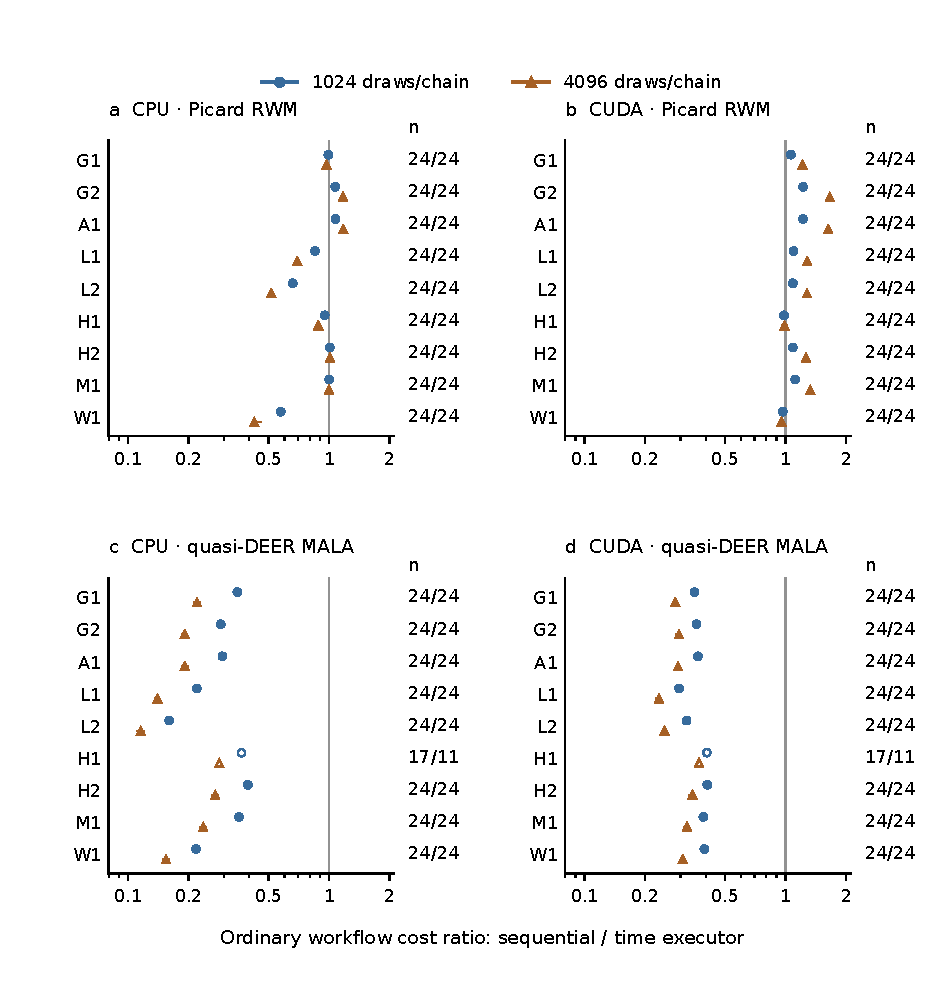
\includegraphics[width=\linewidth]{figures/ordinary-cost-overview.pdf}
\caption{v4 正文采用的普通工作流成本图，原图原样复用。$S=T_{\rm seq}/T_{\rm par}$；重复单位为独立四链输入，区间和失败处理依照本报告第3节。成本不含最外层R前端，缓存与审计口径另外记录。}
\end{figure}

\subsection{重复求值与窗口推进}
历史 Mac M4 CPU 的小型机制实验中，G1四链 Picard 窗口16增到64时，平均确认步数的中位数约5.57，基本不变；每个输出转移的前向映射次数由5.50增至20.88，速度比由0.402降至0.170。更宽窗口计算了更多候选位置，却没有同比推进确认前缀。G2单链 quasi-DEER 的平均轮数由11增至22.25，速度比由0.051降至0.027。

这些次数以全部输出转移为分母，包含拒绝自环；前向映射次数不是浮点工作量，quasi-DEER 的 JVP 成本还另外存在。Windows 机制探测每模型/执行方案只有两份实际输入，分阶段计时可能扰动被测执行，适合解释工作组成，不能构成所有配置减速的精确因果分解。线程设置和向量化也不证明物理核得到有效独占利用。

\subsection{历史负结果与不移动反例}
历史 Mac 主网格1920项中，两种时间执行器所有模型—预算组的缓存中位数均未加速。第一轮 Windows 512项短实验的 CUDA Picard 缓存组中位速度比为1.097--5.230，quasi-DEER为0.164--0.505；每格四份实际输入，属于探索性结果，不以大量 bootstrap 重抽扩大信息量。

第一轮 A1/RWM 的 CUDA Picard 缓存速度比约4.09，但该配置全部拒绝，链停留在初值。执行器因重复状态而一次确认整个窗口，获得较快执行却没有后验探索。正式研究后来独立选择合理步长，原反例仍保留，用于说明执行速度和统计价值的区别；不能把不同批次或缓存/普通口径直接合并。

\section{固定预算误差、应用与探索}
\subsection{误差—成本关系}
式\eqref{eq:loss}固定函数、尺度和参考。两种同核执行在通过核验时提供相同指定路径的统计信息，差异主要为执行成本；跨核比较同时反映局部移动、预热和预算。只测1024/4096两个预算点，连线用于阅读，不代表中间预算已观测，更不估计精确达标时间。

L1/L2 的4096预算 CPU MALA与 CPU NUTS 对比只有六份共同有效重复，未达到20份区间计算下限。原参考共同偏移 $\pm2$ MCSE 内，L1四函数及L2前三函数的点损失差仍保持 NUTS 较小，但这一假设偏移范围不是置信区间，也不能排除有限参考的共同偏差。L2事件原参考与诊断仍未定。

\begin{figure}[p]\centering
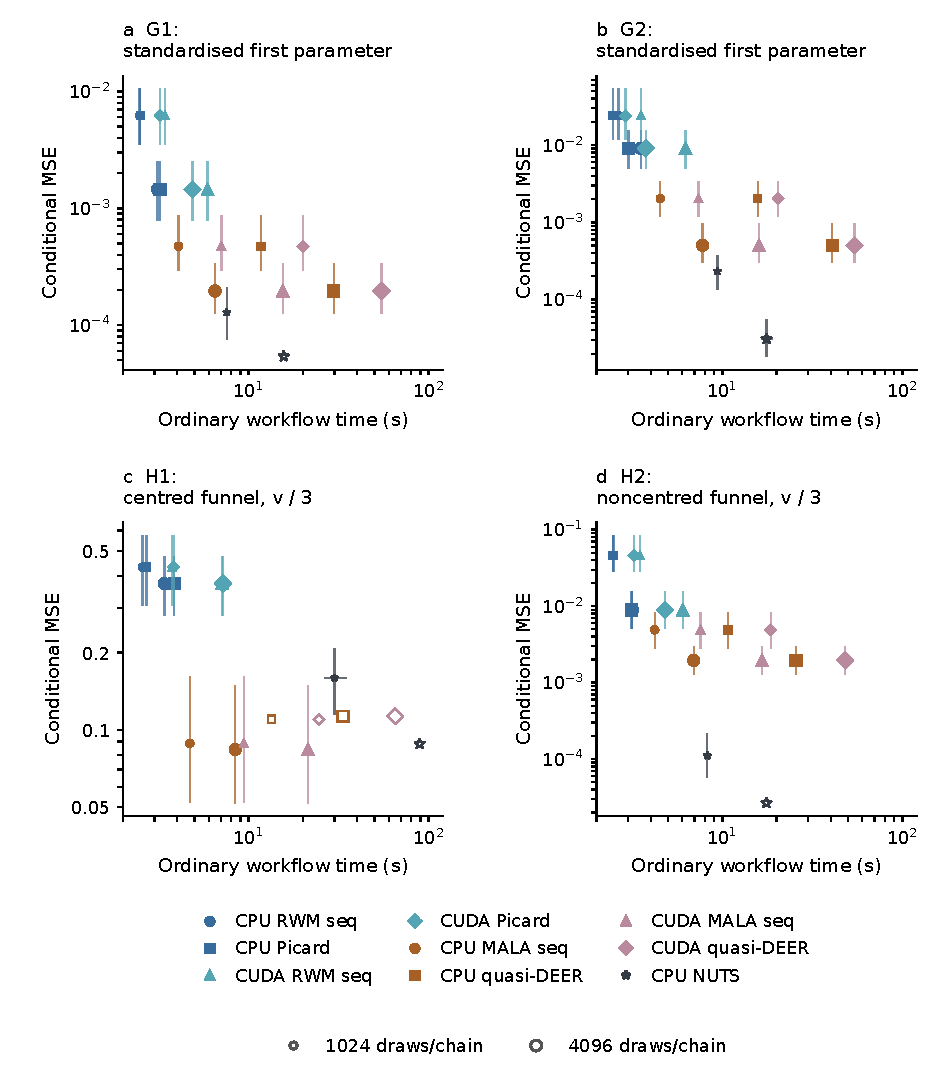
\includegraphics[width=\linewidth]{figures/error-cost-overview.pdf}
\caption{v4 的代表性目标固定预算误差—成本图。四面板是事后解释性展示选择，全部36函数仍按冻结定义报告。沿用原函数和参考，两个预算点之间没有新增观测。完整九目标逐函数结果保存在原67页结果附录。}
\end{figure}

\subsection{水井真实数据 W1}
W1以距离（单位100米）解释换井概率，共3020条记录、截距与距离系数两参数。模型后验可正规化的依据是：存在两个不同距离 $a\ne b$，各有相反结局；取四条相应观测，其余似然因子不超过1。记 $g(v)=\sigma(v)\{1-\sigma(v)\}$，则
\begin{equation}
L(\alpha,\beta)\leq g(\alpha+a\beta)g(\alpha+b\beta),\qquad
\int_{\R^2}L\,d\alpha\,d\beta\leq\frac{1}{|b-a|}<\infty.
\end{equation}
等式使用 $\int g(v)dv=1$；具体观测见 v4 补充材料。这是指定二维模型的论证，不扩展到任意平坦先验回归。

\begin{table}[htbp]\centering\small
\begin{tabular}{lrrr}\toprule
工作流 & 普通耗时（秒） & $\alpha$参考平方差（$10^{-6}$） & $\beta$参考平方差（$10^{-6}$）\\\midrule
CPU RWM seq & 4.94 & 2.06 [1.16, 3.40] & 4.91 [2.72, 7.94]\\
CPU Picard & 11.59 & 2.06 [1.16, 3.40] & 4.91 [2.72, 7.94]\\
CUDA RWM seq & 5.73 & 2.06 [1.16, 3.40] & 4.91 [2.72, 7.94]\\
CUDA Picard & 6.01 & 2.06 [1.16, 3.40] & 4.91 [2.72, 7.94]\\
CPU MALA seq & 10.58 & 0.58 [0.39, 0.89] & 1.11 [0.68, 2.00]\\
CPU quasi-DEER & 68.85 & 0.58 [0.39, 0.89] & 1.11 [0.68, 2.00]\\
CUDA MALA seq & 13.99 & 0.58 [0.39, 0.89] & 1.11 [0.68, 2.00]\\
CUDA quasi-DEER & 45.51 & 0.58 [0.39, 0.89] & 1.11 [0.68, 2.00]\\
CPU NUTS & 11.62 & 0.28 [0.14, 0.51] & 0.52 [0.32, 0.84]\\
\bottomrule\end{tabular}
\caption{水井W1在每链4096次保留转移下的普通工作流耗时均值和参考平方差。每行24份原始四链重复；方括号为条件95\% BCa区间。表中沿用冻结求积参考点；BCa区间不传播参考误差，后续数值包络分析另列。耗时包含普通进程与R诊断，不含最外层R前端。其余五函数和1024步结果见完整结果附录图R39--R45。}
\label{tab:compact-wells}
\end{table}

4096预算下所有工作流各24份有效重复，六个非稀有函数的 $\hat R$ 均不超过1.01，符号事件仍为常量。MALA对截距及斜率的参考平方差较RWM小；但 quasi-DEER明显增加MALA执行成本。CPU NUTS 在本预算提供更小点参考平方差，并付出自身适应与四进程成本，不能由单一表格推广到所有目标。

\begin{table}[htbp]\centering\smalltable
\begin{tabular}{lrrr}\toprule
参数/概率 & 参考样本后验均值 & 95\%等尾后验区间 & 均值 MCSE\\\midrule
$\alpha$ & 0.606710 & [0.488359, 0.723356] & $6.33\times10^{-4}$\\
$\beta$ & -0.622143 & [-0.810761, -0.429960] & 0.00104\\
$p(0)$ & 0.647069 & [0.619720, 0.673346] & $1.44\times10^{-4}$\\
$p(100)$ & 0.496146 & [0.465215, 0.526176] & $1.58\times10^{-4}$\\\bottomrule
\end{tabular}
\caption{独立既有 Stan 参考的应用摘要。10链各保存1000个相关状态；分位数未另量化计算误差。后验区间与均值 MCSE 描述不同不确定性。}
\end{table}
在这个指定模型中，距离较远与较低换井概率相关，不能解释为距离的因果效应。表中有限样本后验均值与确定求积点略不同，来源和 MCSE 一并保留。

\subsection{多峰目标 M1}
有效412项 M1 拟合中，411项没有保存状态的首坐标符号跨越；包括384项MH和28项NUTS有效任务。四链初值两条在每个峰，池化符号比例可以恰为1/2，即使每条链停留在各自模式。唯一保存跨越出现在短预算 NUTS 第5份输入的第3链；池化正比例0.614990234375，该链正比例0.4599609375。20项失败没有被纳入这些比率，也不由保存状态推测未保存的 HMC 积分轨迹。

\begin{figure}[p]\centering
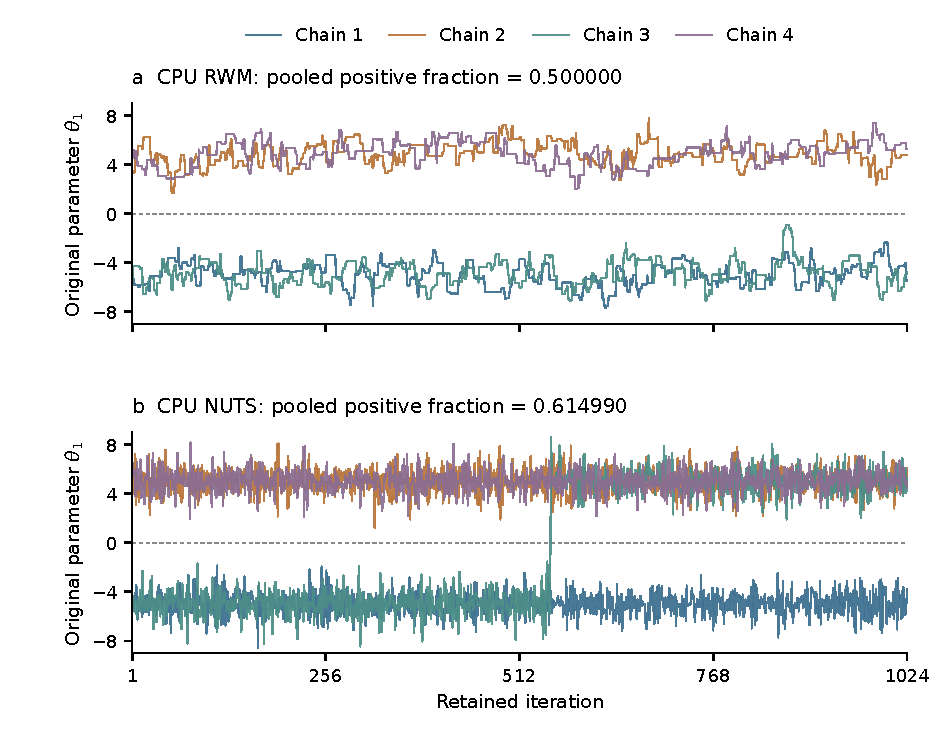
\includegraphics[width=\linewidth]{figures/mixture-example.pdf}
\caption{v4 的 M1 探索示例，保留原图。均衡初始化下池化比例接近真值不能替代跨峰探索；保存转移、逐链行为与失败分母共同解释。}
\end{figure}

\section{有限补充的结果与解释}
\subsection{H1 函数路径差：小均值差不改变失败资格}
H1伴随分析读取80项原任务，其中42失败、38配对有效，共3200个函数分析行、1,130,496次转移。接受事件与符号函数均无失配，四个函数的最大逐点差与池化均值差如下。
\begin{table}[htbp]\centering\smalltable
\begin{tabular}{lrrr}\toprule
函数 & 最大逐点差 & 最大池化均值差 & 最大单链均值差\\\midrule
$v/3$ & $1.90956\times10^{-3}$ & $1.07757\times10^{-7}$ & $4.35023\times10^{-7}$\\
$\tanh(v/3)$ & $1.45182\times10^{-3}$ & $4.68970\times10^{-8}$ & $1.90353\times10^{-7}$\\
$\ind(x_1>0)$ & 0 & 0 & 0\\
$\cos(x_1e^{-v/2})$ & $3.26872\times10^{-3}$ & $3.07812\times10^{-7}$ & $1.23163\times10^{-6}$\\\bottomrule
\end{tabular}
\caption{原失败与有效路径舍弃512步后的保留段差摘要。均值差取绝对值，池化仅指单任务的四条等长链；各极值可能来自不同任务。参考为独立浮点 NumPy 路径而非精确算术真值。}
\end{table}
函数平均有抵消效应，较小平均差与原状态阈值失配可以同时存在。伴随分析说明所选统计量受影响的量级，没有重新认可原42项失败，也不提供一般后验误差界。

\subsection{CPU NUTS 定位：部分诊断阶段的资源路径}
S2 登记44份四链调用及9份旧诊断作业。资格4/4完成，主体34/36完成，确认2/4完成，旧诊断8/9完成，五次资源停止全部保留。便携21项和原生3项测试通过、无失败或跳过；Mac接收只核验真实原生记录，未在Mac重做Windows Job行为。

所选 G2/A1 四 worker、旧诊断开启配置在1024预热和4096采样后已保存完整样本，最后记录为 \code{legacy_diagnostics_enter}，并收到内存限制消息；关闭旧诊断的预定对照完成。冻结 Pyro 1.9.2 源码给出的临时 float64 数组规模为 $2047\times2047\times64$，对应2,145,387,008字节，每链另有268,173,376字节布尔临时量，多 worker 可能同时分配。这是静态规模，失败栈未直接捕获该笔分配，不作为实测独占峰值。

该对照支持所选失败发生于诊断阶段，不能解释全部105项历史失败。六套旧失败输入在仪表化调用下均完成，故不追溯把105项全改为内存故障。8 GiB RSS与12 GiB Job保护保持原样；旧部分链、资源停止和未分类状态继续保留。

\subsection{W1 确定参考包络}
W1以384位球算术实现 Gauss 与 Simpson 两条有限域求积，配合256个角扇区及逐矩尾部控制。两路线各7/7函数完成；六个连续均值的交集半宽均不超过 $10^{-8}$。稀有概率的向外舍入范围为
\begin{equation}
\Pr(\beta>0)\in[4.7671124,\,4.7673026]\times10^{-11}.
\end{equation}
完整二进制端点对应半宽约 $9.51\times10^{-16}$。球算术与求积依据见\cite{arb,dlmfquadrature}。两路线共享部分尾部和导数论证，数值交集和保存端点重聚合不等于对全部分析证明的独立形式化认证。

Gauss/Simpson叶单元31,533/37,671，共69,204；实际积分回调378,384/828,740次，预先计入共享项与探测的整体预算1,351,046，不把预算记成实际回调数。参考构造16,198.50秒单列，未加入采样器普通比较成本。

432项有效 W1 拟合得到126个单工作流—预算—函数损失包络及504个配对点损失差包络，其中408个保持固定符号、96个恒等平局，无反转或跨零未定项。平局包括六个连续函数各四项同核相同估计的24项，以及符号事件全部72项（含跨核）的共同零频率。这说明指定参考数值误差下点排序稳定；不是统计显著性或同时置信结论。W1所有符号频率仍为零，小平方差约 $2.27\times10^{-21}$ 与100\%相对误差并存。

\subsection{L2 稀有事件的重要性参考}
另立协议冻结两套混合提议，先导选择与正式随机点分开。每提议8个独立 PCG64 批次，每批131072点，总正式点2,097,152，另有16,384先导点排除。每套提议分别合并其8批分子与分母，用总分子除以总分母，批次联合协方差给出 delta 近似 MCSE，不平均批次比值，也不合并两套提议\cite{owen}。
\begin{table}[htbp]\centering\smalltable
\begin{tabular}{lrr}\toprule
量 & 提议 Q1 & 提议 Q2\\\midrule
$\Pr(\theta_1>0)$估计 & $1.56547893\times10^{-9}$ & $1.76047974\times10^{-9}$\\
近似 MCSE & $5.69091\times10^{-12}$ & $1.24421\times10^{-10}$\\
相对 MCSE & 0.364\% & 7.067\%\\
事件权重 ESS & 176551.83 & 220.20\\
分母权重 ESS & 356889.74 & 161503.98\\
最大归一化事件权重 & 0.000772858 & 0.0248562\\\bottomrule
\end{tabular}
\caption{L2 独立有限重要性参考。两种 ESS 是权重质量描述，不能当作独立重复数或认证精度。Q2事件权重更集中。}
\end{table}
96个保存点独立重新计算的最大对数权重差为 $3.63798\times10^{-12}$，恢复新增随机点为零。该检查支持保存权重的一致性，不保证 MCSE 的有限样本覆盖或排除遗漏尾部。

原414项有效 L2 拟合全部事件频率为零，相对两套正概率估计误差均为100\%；对应条件平方差为 $2.45072\times10^{-18}$ 和 $3.09929\times10^{-18}$。两提议给出不同结果及质量，分别保留，不用新增参考掩盖原18项失败、常量诊断和原事件参考未定。

\subsection{为什么全零未必是混合失败}
用一个明确假想的 IID 参照解释事件频率的分辨率：L2 有4,128,768个保存条目，按 Q1 概率假想全部独立且来自正确后验，期望命中0.0064635、零命中概率99.356\%；W1有4,423,680条目，期望命中0.000210886、零命中概率99.979\%。实际状态链内相关，同核及跨设备还共享轨迹，不能把上述概率当作真实运行概率，条目总数也不是独立样本量。

它们说明极小事件在该预算下缺少有用相对精度，不说明仅凭全零即可判定混合差。诊断、参考与应用精度需分别判断，不能为获得“全部函数达标”而删除稀有函数。

\clearpage
\section{R 使用、扩展与实际调用成本}
\subsection{公开接口的完整短例}
以下调用已经在独立安装目录验证，Python核心为0.2.0.dev2、R安装候选0.2.0.9002。需要按依赖锁选定Python环境，然后在R运行：
\begin{lstlisting}[language=R]
library(parallelbayes)
model <- pb_model("gaussian", dimension = 2L, backend = "torch")
pb_capabilities(model)
stopifnot(pb_validate(model)$passed)
configs <- lapply(c("sequential", "online_picard"), function(executor)
  list(kernel = "rwm", executor = executor, device = "cpu",
       draws = 128L, chains = 4L, step_size = 0.4,
       window = 16L, seed = 2026L, audit = TRUE))
fits <- pb_benchmark(model, configs)
\end{lstlisting}
实际输入标识和接受数组相同，独立参考通过；短链 $\hat R$ 仍可为1.22或1.44。软件正确返回不等于短例已经适合推断。完整脚本见 \code{examples/paper-api.R}；Poisson扩展示例说明如何提供目标、解析梯度与独立 NumPy 参考后，再由R调用。接口对不支持组合明确报错。

\subsection{首次调用与再次调用}
原技术计时为同一 Poisson 实际输入、两参数、32观测、四链各128步，共32个串行新R进程、64次调用。每格四次技术重复；首次边界包括最外层 R 启动和依赖导入，再次调用仍含采样、传回、转换及诊断，不等于缓存内核计时。
\begin{table}[htbp]\centering\small
\begin{tabular}{llrr}\toprule
模式 & 工作流 & R启动至首次结果/秒 & 会话内再次调用/秒\\\midrule
普通 & RWM / 顺序 & 1.274 [1.267, 1.282] & 0.014 [0.014, 0.015]\\
普通 & RWM / Picard & 1.274 [1.270, 1.315] & 0.014 [0.013, 0.014]\\
普通 & MALA / 顺序 & 1.768 [1.691, 5.220] & 0.044 [0.043, 0.045]\\
普通 & MALA / quasi-DEER & 2.057 [2.023, 2.248] & 0.340 [0.335, 0.347]\\
审计 & RWM / 顺序 & 1.277 [1.276, 1.287] & 0.019 [0.019, 0.020]\\
审计 & RWM / Picard & 1.281 [1.274, 1.358] & 0.019 [0.019, 0.020]\\
审计 & MALA / 顺序 & 1.712 [1.696, 1.949] & 0.054 [0.053, 0.057]\\
审计 & MALA / quasi-DEER & 2.041 [2.036, 2.196] & 0.350 [0.346, 0.353]\\
\bottomrule\end{tabular}
\caption{M4 CPU上的R前端技术计时。每格四次串行新进程，给出中位数及最小--最大值；同一实际Poisson输入，四链各128步。首次结果边界含启动和依赖载入，再次调用仍含采样、传输、转换和诊断；完整证据写盘另记。技术重复不增加正式研究的独立样本量，未构造统计区间。}
\label{tab:r-frontend}
\end{table}

启动依赖对短任务占据较大比例，会话复用减少这部分成本；quasi-DEER在短例中仍有明显额外计算。5.220秒的慢首次 MALA 调用保留，未以环境波动删去。表中技术重复没有增加正式主研究的独立输入数，也不使用 BCa 推断更广泛性能。完整证据写盘另计。

\section{独立接收、重建与投稿候选}
\subsection{主研究的 Mac 接收}
Windows紧凑交付21组件、232,755文件，共29,311,383,786字节，接收时全部完整性通过；253个冻结源码文件与交付源匹配。独立读取全部4144份原始任务/缓存记录，读取错误零；按原身份恢复新增执行零，42,035项检查对象保持原样。

跨系统1132个浮点统计值最大尺度化差 $7.51\times10^{-15}$；4589个 bootstrap 数组中4566逐位相同，其余最大差 $6.67\times10^{-16}$，NaN与分类一致。现代R诊断最大差 $4\times10^{-14}$，未改变 $\hat R$ 阈值结论。末位浮点差作为具体核对结果记录，不扩展为任意平台逐位复现承诺。

\subsection{统一材料与内部验收}
投稿候选的41组件清单列示39,354,532,214字节，约36.65 GiB；包含重叠历史归档，不能把字节数理解为独立科学信息。轻量入口包含源码 bundle、论文输入、安装候选、传输清单与验收记录，原始大组件另外提供。旧CPU原件在既有 Release，Windows原件在未公开草稿，本地 H1/L2/W1 原件按清单定位；不把草稿URL称为匿名审稿访问入口。

同一Mac的新Python分析环境和新解包目录完成内部重建，14项分析依赖固定且 \code{pip check} 通过，未导入推断后端重新采样。从4144份已有分析记录重新计算统计，4589个 bootstrap 数组完全一致；81个主CSV、4个补充CSV、6个主文片段及45幅图一致。保存的L2点重权与W1端点重聚合另行核对，没有重新生成正式点或积分回调。

原169个LaTeX内容输入匹配，正文18页及SI45页重编译后，全部63页文本与72 dpi像素相同，无未解析引用或超宽；原67页完整结果附录未改。新wheel与R源码包安装核验17个模块，并完成两次CPU技术调用；R依赖库明确复用原锁定库，GPU未重测。归档工具7项测试通过、无失败/跳过，检查损坏、成员异常、路径逃逸和预算保护，不作为 MCMC 数学正确性证据。

首次环境导入及初始软件依赖闭包曾失败，日志保留；补齐实际 psutil/SciPy 等依赖后通过，冻结采样核心未改。本轮是内部新环境与目录验收，不是外部团队、全新R生态或异机复现；从保存记录重聚合也不是第二次全量路径重放。

\subsection{固定版本与尚待作者确认的事项}
紧凑执行源 \code{3a37a89}、交付源 \code{94bebec}；中文v4构建源 \code{699e645}；投稿候选 \code{b84e966}，标签 \code{submission-v4-rc1}。源码、协议、保存数组、版本差异和完整性清单分别绑定，历史0.1.0/0.1.1不被覆盖。本报告仅新增说明文档及其PDF，不更新原科学结果。

作者须确认署名/单位/通讯、资助/利益冲突、数据权利与公开范围、真实审稿访问路线、期刊/语言与AI披露，以及最终批准。非作者或匿名权限下的实际材料下载尚未验收；代码仓库可取得不等于全部证据公开。项目不自动公开原私有草稿，不自动提交期刊或CRAN。

\section{讨论与研究完成边界}
时间并行的收益取决于每轮批量计算节省的时间能否抵消重复求值、导数、扫描与控制成本。本研究中 quasi-DEER 未达到这一条件；Picard 在部分 CUDA 组达到同核普通执行收益，仍须结合后验函数与逐链探索解释。大窗口增加候选工作而不一定增加确认进展，全拒绝轨迹和均衡双峰初始化则揭示执行与探索的不同。

有限参考会改变误差比较的含义。L2重要性参考以近似MCSE与权重质量描述，W1确定包络限定数值参考误差；二者都不能替代正式重复的不确定性。稀有事件的绝对精度与相对精度差异说明函数选择及尺度必须先明确，不能把一个统一数值阈值解释为所有应用的同等可靠性。

本研究的局限是当前实现含主机控制、目标库未系统覆盖真正昂贵黑箱似然、只测两个预算、部分NUTS任务失败且原因未全分类、有限重要性参考可能存在尾部遗漏，以及系统资源不是独占物理核预算。后续若研究融合执行、昂贵目标或配置选择，应设新协议，不改写现有负结果。

当前规定范围内的软件、研究计算、伴随分析和内部重建已经完成。投稿准备主要剩余作者信息、材料访问与期刊适配；不需要为证明普遍加速增加网格。最终文章应由当前证据支持的计算与探索结论组成，并由作者审定其适用范围。

\clearpage
\appendix
\section{报告内容与 v4 来源的对应}
\begin{longtable}{P{36mm}P{108mm}}
\caption{随 LaTeX 包提供的来源映射另保存完整哈希。下表给出逻辑位置，避免依赖本机绝对目录。}\\
\toprule 报告内容 & 冻结来源（相对项目根目录）\\\midrule\endfirsthead
\toprule 报告内容 & 冻结来源（相对项目根目录）\\\midrule\endhead
方法与能力 & \code{manuscript/software/软件与基准研究.tex}，方法及软件设计节\\
模型与步长 & \path{manuscript/software/revision-configuration.generated.tex}\\
主要计数与速度比 & \path{compact-scalars.generated.tex}、\path{compact-outcomes.generated.tex}\\
参考及水井应用 & \path{revision-reference.generated.tex}、\path{compact-wells.generated.tex}\\
H1、L2、W1补充 & \path{targeted-h1-main.generated.tex}、\path{targeted-l2-si.generated.tex}、\path{w1-enclosure-results.tex}及配套伴随分析\\
CPU NUTS定位 & \path{nuts-localization-si.generated.tex}、\path{docs/WINDOWS-NUTS-MAC-REVIEW.md}\\
R前端与IID参照 & \path{r-frontend.generated.tex}、\path{review3-scalars.generated.tex}\\
内部验收与作者事项 & \path{docs/SUBMISSION-RC1.md}、\path{docs/AUTHOR-DECISIONS.md}\\\bottomrule
\end{longtable}
未注明目录的生成片段均位于 \code{manuscript/software/}。本报告复用三幅第一方科学图件，数据、图形与哈希均保留原绑定。

\clearpage% Selected unchanged entries from frozen v4; scientific usage is described in the documents.
\begin{thebibliography}{99}\small\setlength{\itemsep}{3pt}
\bibitem{zoltowski} Zoltowski D.M., Wu S., Gonzalez X., et al. \href{https://proceedings.nips.cc/paper_files/paper/2025/hash/202886ee1c9ca735cb5bff3a00a69883-Abstract-Conference.html}{Parallelizing MCMC Across the Sequence Length}. Advances in Neural Information Processing Systems, 2025, 38.
\bibitem{grazzi} Grazzi S., Zanella G. \href{https://doi.org/10.1093/biomet/asag022}{Parallel computations for Metropolis Markov chains with Picard maps}. Biometrika, 2026, 113(2): asag022.
\bibitem{stan} Carpenter B., Gelman A., Hoffman M.D., et al. \href{https://doi.org/10.18637/jss.v076.i01}{Stan: A Probabilistic Programming Language}. Journal of Statistical Software, 2017, 76(1): 1--32.
\bibitem{bridgestan} Roualdes E.A., Ward B., Carpenter B., Seyboldt A., Axen S.D. \href{https://doi.org/10.21105/joss.05236}{BridgeStan: Efficient in-memory access to the methods of a Stan model}. Journal of Open Source Software, 2023, 8(87):5236.
\bibitem{blackjax} Cabezas A., Corenflos A., Lao J., Louf R., et al. \href{https://arxiv.org/abs/2402.10797}{BlackJAX: Composable Bayesian inference in JAX}. arXiv:2402.10797, 2024.
\bibitem{pyro} Bingham E., Chen J.P., Jankowiak M., et al. \href{https://jmlr.org/papers/v20/18-403.html}{Pyro: Deep Universal Probabilistic Programming}. Journal of Machine Learning Research, 2019, 20(28):1--6.
\bibitem{comparemcmcs} NIMBLE development team. \href{https://github.com/nimble-dev/compareMCMCs}{compareMCMCs: Tools for comparing MCMC efficiency from NIMBLE and other engines}. 软件作者仓库，访问于2026年10月3日。
\bibitem{posterior} Stan development team. \href{https://mc-stan.org/posterior/reference/rhat.html}{posterior: Rhat, bulk ESS and tail ESS documentation}. 软件文档，版本1.7.0。
\bibitem{parallelmcmc} Senne R. and contributors. \href{https://github.com/rsenne/ParallelMCMC.jl/tree/7be9c866c8be03ad994a5e7f0486ec3290088813}{ParallelMCMC.jl}. 软件仓库，提交7be9c86，访问于2026年10月6日。
\bibitem{bayesforge} Sosa S. \href{https://cran.r-universe.dev/BayesForge/doc/manual.html}{BayesForge: Bayesian Inference using numpyro and XLA}. R包0.0.1参考手册，访问于2026年10月6日。
\bibitem{gonzalez} Gonzalez X., Warrington A., Smith J.T.H., Linderman S.W. \href{https://arxiv.org/abs/2407.19115v3}{Towards Scalable and Stable Parallelization of Nonlinear RNNs}. arXiv:2407.19115v3, 2025（初版2024）.
\bibitem{vehtari} Vehtari A., Gelman A., Simpson D., Carpenter B., Bürkner P.-C. \href{https://doi.org/10.1214/20-BA1221}{Rank-Normalization, Folding, and Localization: An Improved R-hat for Assessing Convergence of MCMC}. Bayesian Analysis, 2021, 16(2):667--718.
\bibitem{modrak} Modrák M., Moon A.H., Kim S., et al. \href{https://doi.org/10.1214/23-BA1404}{Simulation-Based Calibration Checking for Bayesian Computation: The Choice of Test Quantities Shapes Sensitivity}. Bayesian Analysis, 2025, 20(2):461--488. DOI:10.1214/23-BA1404.
\bibitem{owen} Owen A.B. \href{https://artowen.su.domains/mc/}{Monte Carlo theory, methods and examples}. 2013, Chapter 9: Importance sampling. 在线书稿。
\bibitem{dlmfquadrature} National Institute of Standards and Technology. \href{https://dlmf.nist.gov/3.5}{Digital Library of Mathematical Functions, Section 3.5: Quadrature}. Equations 3.5.6, 3.5.19--3.5.21，访问于2026年10月10日。
\bibitem{arb} Johansson F. \href{https://doi.org/10.1109/TC.2017.2690633}{Arb: Efficient Arbitrary-Precision Midpoint-Radius Interval Arithmetic}. IEEE Transactions on Computers, 2017, 66(8):1281--1292.
\end{thebibliography}

\end{document}
